% =====================================================================
%  Lógica de la Investigación Social (SOC8123) — UDP, 2° semestre 2026
%  Clase 06/10: Encuestas, cuestionarios y medición
%  Profesor invitado: Alejandro Plaza Reveco
%  Estilo: Manual de Estilo de Presentaciones — Plaza Reveco (2026)
%  Compilar con pdflatex (dos pasadas)
%
%  TIEMPOS SUGERIDOS (80 min)
%   1. Medir y encuestar: lo básico ....................... 12 min
%   2. Obsesionarse con el error (TSE) .................... 18 min
%   3. Del concepto al número (operacionalización) ........ 16 min
%   4. Tres casos reales: ELSOC ........................... 20 min
%   5. Innovaciones: experimentos, modos, datos vinculados  12 min
%   Cierre ............................................... 2 min
%
%  IMÁGENES: \imagen{archivo}{ancho}{alto}{descripción} muestra
%  imagenes/archivo si existe; si no, dibuja un recuadro con la
%  sugerencia. El documento compila igual sin imágenes.
%  Archivos esperados: ver imagenes/LEEME.txt
% =====================================================================

% -- CLASE DEL DOCUMENTO
\documentclass[aspectratio=169,11pt]{beamer}

% -- PAQUETES ESENCIALES
\usepackage[spanish]{babel}
\usepackage[utf8]{inputenc}
\usepackage[T1]{fontenc}
\usepackage{lmodern}
\usepackage{amsmath, amssymb}
\usepackage{booktabs}
\usepackage{xcolor}
\usepackage{graphicx}
\usepackage{array}
\usepackage{colortbl}

% -- TIKZ
\usepackage{tikz}
\usepackage{pgfplots}
\pgfplotsset{compat=1.18}
\usetikzlibrary{arrows.meta, positioning, decorations.pathreplacing, calc, babel}

% -- TEMA
\usetheme{Madrid}
\setbeamertemplate{navigation symbols}{}
\setbeamertemplate{headline}{}
\setbeamertemplate{footline}[frame number]

% -- PALETA PERSONAL (azul marino + dorado, aplazareveco.com)
\definecolor{marino}{HTML}{1B2D4F}       % azul marino principal
\definecolor{dorado}{HTML}{C9A84C}       % dorado acento
\definecolor{acero}{HTML}{2E5073}        % azul acero — alertblock
\definecolor{salvia}{HTML}{6B7C5A}       % verde salvia — exampleblock
\definecolor{crema}{HTML}{EDE8DF}        % crema — filas alternas
\definecolor{doradooscuro}{HTML}{A07830} % dorado oscuro — datos grupo 2
\definecolor{azulmedio}{HTML}{2D6A9F}    % azul medio — datos grupo 1
\definecolor{pizarra}{HTML}{4A5568}      % gris pizarra — datos grupo 3
\definecolor{gris}{HTML}{595959}         % gris neutro

% -- COLORES DEL TEMA
\setbeamercolor{title}{fg=marino}
\setbeamercolor{frametitle}{fg=white,bg=marino}
\setbeamercolor{structure}{fg=marino}
\setbeamercolor{normal text}{fg=black,bg=white}
\setbeamercolor{block title}{fg=white,bg=marino}
\setbeamercolor{block body}{fg=black,bg=marino!6}
\setbeamercolor{block title alerted}{fg=white,bg=acero}
\setbeamercolor{block body alerted}{fg=black,bg=acero!6}
\setbeamercolor{block title example}{fg=white,bg=salvia}
\setbeamercolor{block body example}{fg=black,bg=salvia!8}

% -- FUENTES
\setbeamerfont{title}{series=\bfseries,size=\LARGE}
\setbeamerfont{subtitle}{size=\large}
\setbeamerfont{frametitle}{series=\bfseries,size=\normalsize}

% -- FRAMETITLE personalizado
\setbeamertemplate{frametitle}{
  \nointerlineskip
  \begin{beamercolorbox}[wd=\paperwidth,ht=2.8ex,dp=1ex,
                         leftskip=0.8em]{frametitle}
    \insertframetitle
  \end{beamercolorbox}}

% -- MACROS
\newcommand{\hl}[1]{\textcolor{marino}{\textbf{#1}}}        % enfasis marino
\newcommand{\hlr}[1]{\textcolor{acero}{\textbf{#1}}}        % enfasis acero (alerta)
\newcommand{\hld}[1]{\textcolor{doradooscuro}{\textbf{#1}}} % enfasis dorado
\newcommand{\code}[1]{\texttt{\small #1}}                    % codigo inline
\newcommand{\fuente}[1]{\par\vfill{\scriptsize\color{gris}#1\par}}

\renewcommand{\arraystretch}{1.5}

% -- IMAGEN CON RESPALDO (recuadro si falta el archivo)
\graphicspath{{imagenes/}}
\newcommand{\imagen}[4]{%
  \IfFileExists{imagenes/#1}%
    {\includegraphics[width=#2,height=#3,keepaspectratio]{#1}}%
    {\fcolorbox{gris}{crema!60}{\parbox[c][#3][c]{#2}{\centering\scriptsize\color{gris}%
      \textbf{Imagen sugerida}\\[2pt] #4\\[4pt]\texttt{imagenes/\detokenize{#1}}}}}%
}

% -- SEPARADOR DE SECCIÓN
\newcommand{\seccion}[2]{%
\begin{frame}[plain]
\vspace{2cm}\begin{center}
  {\Large\textbf{\textcolor{marino}{#2}}}\\[0.5cm]
  {\large\color{dorado} #1}
\end{center}
\end{frame}}

% -- DIANA (tiro al blanco)
\newcommand{\diana}[3]{%
    \begin{scope}[shift={(#1,#2)}]
      \foreach \r/\c in {1.6/crema,1.1/marino!20,0.6/marino!40,0.2/marino} \fill[\c] (0,0) circle (\r);
      \draw[pizarra] (0,0) circle (1.6);
      \node[font=\scriptsize, align=center, text=pizarra] at (0,-2.2) {#3};
    \end{scope}}

% -- OVERLAYS EN TIKZ (aparecer de a poco sin mover el dibujo)
\tikzset{
  invisible/.style={opacity=0, text opacity=0},
  visible on/.style={alt={#1{}{invisible}}},
  alt/.code args={<#1>#2#3}{\alt<#1>{\pgfkeysalso{#2}}{\pgfkeysalso{#3}}},
}

% -- ESTILOS TIKZ (rounded corners=4pt, fill=COLOR!15, draw=text)
%    no observada = marino · observada = pizarra · error = dorado oscuro
\tikzset{
  every picture/.style={font=\sffamily, >=Stealth},
  lat/.style={draw=marino, text=marino, fill=marino!15, thick, rounded corners=4pt,
              minimum width=2.4cm, minimum height=0.9cm, font=\sffamily\small\bfseries, align=center},
  obs/.style={draw=pizarra, text=pizarra, fill=pizarra!15, thick, rounded corners=4pt,
              minimum width=2.2cm, minimum height=0.8cm, font=\sffamily\small, align=center},
  errn/.style={draw=doradooscuro, text=doradooscuro, fill=doradooscuro!15, thick, rounded corners=4pt,
              minimum width=1.6cm, minimum height=0.8cm, font=\sffamily\small\bfseries, align=center},
  flecha/.style={-Stealth, thick, pizarra},
  flechae/.style={-Stealth, thick, doradooscuro},
  flechad/.style={-Stealth, thick, dashed, doradooscuro},
}

% -- METADATOS
\title{Encuestas, cuestionarios y medición}
\subtitle{Del concepto al número: trabajar con el error}
\author{Alejandro Plaza Reveco}
\institute{Sociología UDP}
\date{6 de octubre de 2026}

% -- PORTADA (idéntica al inicio y al final)
\newcommand{\portada}{%
\begin{frame}[plain]
  \vspace{0.5cm}
  {\usebeamerfont{title}\color{marino}\inserttitle\par}
  \vspace{0.2cm}
  {\usebeamerfont{subtitle}\color{gris}\insertsubtitle\par}
  \vspace{0.3cm}
  {\color{dorado}\rule{0.6\textwidth}{1pt}\par}
  \vspace{0.6cm}
  {\insertauthor\ (profesor invitado)\par}\vspace{0.1cm}
  {\small Lógica de la Investigación Social · Sociología --- Universidad Diego Portales\par}\vspace{0.1cm}
  {\insertdate\par}
\end{frame}}

% -- SÍNTESIS (fondo marino, texto dorado)
\newcommand{\sintesis}[1]{%
{\setbeamercolor{background canvas}{bg=marino}
\setbeamercolor{itemize item}{fg=dorado}
\begin{frame}[plain]
\vspace{0.6cm}
{\large\color{dorado}\textbf{Síntesis}\par}
\vspace{0.4cm}
\begin{itemize}
#1
\end{itemize}
\end{frame}}}

% =====================================================================
\begin{document}
% =====================================================================

\portada

% ---------------------------------------------------------------------
\begin{frame}{Hoja de ruta}
\begin{enumerate}
  \item \textbf{Medir y encuestar: lo básico} --- variables, niveles de medición, cuestionarios
  \item \textbf{Obsesionarse con el error} --- nos vamos a equivocar: ¿por cuánto?
  \item \textbf{Del concepto al número} --- conceptos latentes y operacionalización
  \item \textbf{Tres casos reales (ELSOC)}
    \begin{itemize}
      \item Autoeficacia política: una escala corta, varias facetas
      \item Autoritarismo: cuando el formato empuja las respuestas
      \item Depresión: cuando la situación empuja las respuestas
    \end{itemize}
  \item \textbf{Innovaciones} --- experimentos, modos de aplicación y datos vinculados
\end{enumerate}
\end{frame}

% =====================================================================
\seccion{Parte 1}{Medir y encuestar: lo básico}

% ---------------------------------------------------------------------
\begin{frame}{¿Qué significa medir?}
\begin{columns}[c]
\column{0.55\textwidth}
\begin{block}{Definición clásica}
\small
Medir es \hl{asignar números a objetos o eventos según reglas} (Stevens, 1946)
\end{block}
\bigskip
\begin{itemize}
  \item Medimos estatura con una regla, temperatura con un termómetro
  \item En sociología medimos edad, ingreso, confianza, autoritarismo\ldots
  \item La pregunta de hoy: ¿con qué \textbf{regla} le asignamos un número a la confianza en las instituciones?
\end{itemize}
\column{0.4\textwidth}
\centering
\begin{tikzpicture}[scale=0.9]
  \node[lat] (c) at (0,2.4) {Concepto\\\footnotesize\mdseries ``confianza''};
  \node[obs] (r) at (0,0.9) {Regla\\\footnotesize (pregunta + escala)};
  \node[errn, draw=marino, text=marino, fill=marino!15, minimum width=2.2cm] (n) at (0,-0.6) {Número\\\footnotesize\mdseries 1, 2, 3, 4, 5};
  \draw[flecha] (c) -- (r); \draw[flecha] (r) -- (n);
\end{tikzpicture}
\end{columns}
\fuente{Stevens, S. S. (1946). On the theory of scales of measurement. \emph{Science}, 103(2684).}
\end{frame}

% ---------------------------------------------------------------------
\begin{frame}{¿Qué es una variable?}
\begin{block}{Definición}
\small
Una \hl{variable} es una característica que \textbf{toma distintos valores} entre las unidades que estudiamos (personas, hogares, comunas\ldots)
\end{block}
\bigskip
\begin{center}
\small
\begin{tabular}{lllcr}
\toprule
\textbf{Persona} & \textbf{Comuna} & \textbf{Nivel educacional} & \textbf{Confianza (1--5)} & \textbf{Edad} \\
\midrule
\rowcolor{crema}
Ana    & Maipú        & Media completa   & 2 & 34 \\
Benito & Ñuñoa        & Universitaria    & 4 & 51 \\
\rowcolor{crema}
Carla  & Temuco       & Básica           & 3 & 67 \\
Diego  & Antofagasta  & Técnica superior & 1 & 22 \\
\bottomrule
\end{tabular}
\end{center}
\bigskip
\begin{itemize}
  \item Cada fila es una \textbf{unidad}; cada columna, una \textbf{variable}
  \item ¿Las cuatro columnas son ``datos'' del mismo tipo?
\end{itemize}
\end{frame}

% ---------------------------------------------------------------------
\begin{frame}{Niveles de medición}
\begin{center}
\small
\renewcommand{\arraystretch}{1.6}
\begin{tabular}{>{\raggedright}p{0.15\textwidth}>{\raggedright}p{0.3\textwidth}>{\raggedright}p{0.25\textwidth}p{0.2\textwidth}}
\toprule
\textbf{Nivel} & \textbf{Qué nos dicen los valores} & \textbf{Ejemplos} & \textbf{Operaciones} \\
\midrule
\rowcolor{crema}
\textbf{Nominal} & Solo \textbf{categorías distintas}, sin orden & Comuna, partido, sexo & Contar \\
\textbf{Ordinal} & Categorías \textbf{con orden}, pero distancias desconocidas & Nivel educacional, escala de acuerdo & Contar, ordenar \\
\rowcolor{crema}
\textbf{Continua} & \textbf{Distancias iguales}: un año más es siempre un año más & Edad en años, ingreso, horas de trabajo & Contar, ordenar, sumar, promediar \\
\bottomrule
\end{tabular}
\end{center}
\bigskip
\begin{alertblock}{Ojo}
\small
El número que ponemos en la base de datos \textbf{no cambia} el nivel de medición: codificar ``Norte = 1, Centro = 2, Sur = 3'' no convierte la zona en una variable numérica
\end{alertblock}
\end{frame}

% ---------------------------------------------------------------------
\begin{frame}{Asignar números a conceptos: un ejemplo}
\begin{columns}[T]
\column{0.5\textwidth}
``¿Cuánto confía usted en el Congreso?''
\bigskip

\centering
\begin{tikzpicture}[scale=0.9]
  \foreach \t/\n [count=\i] in {Nada/1, Poca/2, Algo/3, Bastante/4, Mucha/5} {
    \node[obs, minimum width=1.9cm, minimum height=0.55cm] (c\i) at (0,-\i*0.8) {\t};
    \node[lat, minimum width=0.8cm, minimum height=0.55cm] (n\i) at (2.8,-\i*0.8) {\n};
    \draw[flecha] (c\i) -- (n\i);
  }
\end{tikzpicture}
\column{0.46\textwidth}
\begin{itemize}
  \item Los números respetan el \textbf{orden}: más número, más confianza
  \item Pero, ¿la distancia entre ``Nada'' y ``Poca'' es igual a la de ``Bastante'' y ``Mucha''?
  \item Si lo es, podemos \hl{promediar}; si no, es una variable ordinal
\end{itemize}
\bigskip
\begin{exampleblock}{Para pensar}
\small
Un promedio de confianza de 2,4: ¿qué significa exactamente?
\end{exampleblock}
\end{columns}
\end{frame}

% ---------------------------------------------------------------------
\begin{frame}{Ejercicio rápido: ¿qué nivel de medición?}
\begin{columns}[T]
\column{0.55\textwidth}
\begin{enumerate}
  \item Edad en años cumplidos
  \item Edad en tramos: 18--29, 30--44, 45--64, 65+
  \item Comuna de residencia
  \item Satisfacción con la vida, de 1 a 10
  \item Número de amigos cercanos
  \item Candidato por el que votó
\end{enumerate}
\column{0.4\textwidth}
\begin{block}{Pista}
\small
Pregúntense: ¿tiene orden? ¿Las distancias son iguales?
\end{block}
\bigskip
\begin{alertblock}{Una decisión de diseño}
\small
La \textbf{misma} variable (edad) puede medirse a distintos niveles: preguntar en tramos \textbf{pierde información}
\end{alertblock}
\end{columns}
\end{frame}

% ---------------------------------------------------------------------
\begin{frame}{Un cuestionario, según Asún}
\begin{block}{Definición}
\small
``Un cuestionario es un dispositivo de investigación cuantitativa consistente en un conjunto de preguntas que deben ser aplicadas a un sujeto (usualmente individual) en un orden determinado y frente a las cuales este sujeto puede responder adecuando sus respuestas a un espacio restringido o a una serie de respuestas que el mismo cuestionario ofrece.''
\end{block}
\bigskip
\begin{itemize}
  \item Objetivo: \hl{``medir'' el grado o la forma} en que las personas poseen determinadas variables
  \item Es una \textbf{conversación no horizontal}: uno pregunta con opciones preestablecidas, el otro elige
\end{itemize}
\fuente{Asún (2006, p.~67).}
\end{frame}

% ---------------------------------------------------------------------
\begin{frame}{Encuesta $\neq$ cuestionario}
\centering
\begin{tikzpicture}[scale=0.9]
  \node[obs, minimum width=3.3cm, minimum height=1.3cm] (q) at (-4.3,0) {\textbf{Cuestionario}\\\footnotesize ¿qué preguntamos\\\footnotesize y cómo?};
  \node[obs, minimum width=3.3cm, minimum height=1.3cm] (m) at (0,0) {\textbf{Muestra}\\\footnotesize ¿a quiénes\\\footnotesize preguntamos?};
  \node[obs, minimum width=3.3cm, minimum height=1.3cm] (mo) at (4.3,0) {\textbf{Modo}\\\footnotesize ¿cómo llega\\\footnotesize la pregunta?};
  \node[lat, minimum width=5cm] (e) at (0,-2.2) {Encuesta};
  \draw[flecha] (q) -- (e); \draw[flecha] (m) -- (e); \draw[flecha] (mo) -- (e);
\end{tikzpicture}
\bigskip
\begin{itemize}
  \item Un buen cuestionario aplicado a una mala muestra produce \textbf{malos datos}
  \item Una muestra perfecta con preguntas mal hechas, \textbf{también}
  \item Modos: cara a cara, teléfono, web, autoaplicado\ldots\ o \hl{mezclas}
\end{itemize}
\end{frame}

% ---------------------------------------------------------------------
\begin{frame}{¿Qué se puede preguntar?}
\begin{columns}[T]
\column{0.32\textwidth}
\begin{block}{Hechos}
\small
Conductas o sucesos\\[3pt]
\footnotesize ¿Votó en la última elección? ¿Con quién vive?
\end{block}
\column{0.32\textwidth}
\begin{block}{Conocimientos y habilidades}
\small
Hay respuestas correctas e incorrectas\\[3pt]
\footnotesize Pruebas SIMCE o PAES, preguntas de conocimiento político
\end{block}
\column{0.32\textwidth}
\begin{block}{Opiniones y valores}
\small
Lo que la persona piensa o siente\\[3pt]
\footnotesize ¿Cuánto confía en el Congreso? ¿Qué es más importante: libertad o igualdad?
\end{block}
\end{columns}
\bigskip
\begin{alertblock}{Incluso los hechos pasan por la persona}
\small
Lo que recibimos ``no es el hecho'', sino ``la percepción, recuerdo o lo que nos desea transmitir el sujeto'' (Asún, 2006, p.~78)
\end{alertblock}
\end{frame}

% ---------------------------------------------------------------------
\sintesis{
  \item\textcolor{dorado}{Medir es asignar números a conceptos según una regla explícita}
  \bigskip
  \item\textcolor{dorado}{Las variables pueden ser nominales, ordinales o continuas: el nivel define qué operaciones tienen sentido}
  \bigskip
  \item\textcolor{dorado}{El cuestionario es la regla de medición; la encuesta suma muestra y modo de aplicación}
}

% =====================================================================
\seccion{Parte 2}{Obsesionarse con el error}

% ---------------------------------------------------------------------
\begin{frame}[plain]
\vfill
\begin{center}
{\Large Trabajar con datos cuantitativos significa\par}
\vspace{0.4cm}
{\color{marino}\Huge\bfseries obsesionarse con el error\par}
\vspace{0.3cm}
{\color{dorado}\rule{0.4\textwidth}{1pt}\par}
\vspace{0.5cm}
{\large ¿De dónde viene el error?\par\smallskip
¿Cómo lo evitamos o reducimos?\par\smallskip
¿Cómo le ponemos un \hld{número}?\par}
\end{center}
\vfill
\end{frame}

% ---------------------------------------------------------------------
\begin{frame}{No es si nos equivocamos, sino por cuánto}
\begin{columns}[T]
\column{0.6\textwidth}
\small
Marzo de 2026: debate sobre el MEPCO (Mecanismo de Estabilización de Precios de los Combustibles)
\bigskip

\begin{block}{Mirada determinista}
\small
``El 48\% de los chilenos opina que el Gobierno debía endeudarse para mantener el subsidio del MEPCO''
\end{block}
\bigskip
\begin{exampleblock}{Mirada probabilística}
\small
``Entre \textbf{44\% y 52\%} lo opina, con 95\% de confianza''\\
\footnotesize (ilustrativo: muestra de $\approx$700 casos, margen de $\pm$3,7 puntos)
\end{exampleblock}
\column{0.36\textwidth}
\centering
\imagen{mepco.jpg}{\textwidth}{4.6cm}{Foto asociada al MEPCO: precios en una bencinera o titular del alza}
\end{columns}
\fuente{Dato: Cadem, Plaza Pública (marzo 2026).}
\end{frame}

% ---------------------------------------------------------------------
\begin{frame}{La pregunta científica}
\begin{itemize}
  \item No asumimos que la realidad social se puede capturar sin falla
  \item Asumimos que \hl{nos vamos a equivocar siempre}: por el muestreo, las preguntas, los encuestadores, el procesamiento
  \item La pregunta es: \textbf{¿por cuánto y en qué dirección?}
\end{itemize}
\vspace{0.8cm}
\begin{center}
\begin{minipage}{0.8\textwidth}
\large\itshape
``Medir conceptos de ciencias sociales siempre incorpora un grado variable, pero frecuentemente importante, de error. Equivale a tratar de comprender una conversación escuchada en una radio con mucha estática y ruido de fondo.''
\end{minipage}
\end{center}
\begin{flushright}\small Asún (2006, p.~112)\end{flushright}
\end{frame}

% ---------------------------------------------------------------------
\begin{frame}{El tiro al blanco}
\begin{columns}[c]
\column{0.45\textwidth}
\centering
\begin{tikzpicture}[scale=1.25]
  \diana{0}{0}{}
  \draw[-Stealth, thick, doradooscuro] (2.1,1.3) node[above, font=\small, text=doradooscuro, align=center] {centro =\\valor verdadero} -- (0.25,0.12);
\end{tikzpicture}
\column{0.5\textwidth}
\begin{itemize}
  \item El \hl{centro} es lo que queremos conocer: el valor verdadero en la población
  \item Cada \textbf{disparo} es una medición: una encuesta, una muestra, una respuesta
  \item Nunca vemos el centro directamente: solo vemos dónde caen los disparos
\end{itemize}
\end{columns}
\end{frame}

% ---------------------------------------------------------------------
\begin{frame}{Dos tipos de error}
\centering
\begin{tikzpicture}[scale=0.56]
    \begin{scope}[visible on=<1->]\diana{0}{0}{\textbf{Preciso e insesgado}\\ el ideal}
    \foreach \x/\y in {0.12/0.15,-0.15/0.05,0.05/-0.15,-0.05/-0.1,0.15/-0.02} \filldraw[fill=dorado, draw=white, thick] (\x,\y) circle (0.14);\end{scope}
  \begin{scope}[visible on=<2->]\diana{5}{0}{\textbf{Impreciso, insesgado}\\ error aleatorio}
    \foreach \x/\y in {0.9/0.5,-0.8/0.7,0.4/-1.0,-1.0/-0.4,0.2/1.1,-0.3/-0.9} \filldraw[fill=dorado, draw=white, thick] (5+\x,\y) circle (0.14);\end{scope}
  \begin{scope}[visible on=<3->]\diana{10}{0}{\textbf{Preciso, sesgado}\\ error sistemático}
    \foreach \x/\y in {0.9/0.9,1.05/0.8,0.85/1.05,1.0/1.0,0.95/0.75} \filldraw[fill=dorado, draw=white, thick] (10+\x,\y) circle (0.14);\end{scope}
  \begin{scope}[visible on=<4->]\diana{15}{0}{\textbf{Impreciso y sesgado}\\ lo peor}
    \foreach \x/\y in {1.1/0.3,0.4/1.2,1.3/1.1,0.6/0.5,1.0/-0.1,0.2/0.9} \filldraw[fill=dorado, draw=white, thick] (15+\x,\y) circle (0.14);\end{scope}
\end{tikzpicture}
\bigskip
\begin{itemize}
  \item<1-> \textbf{El ideal}: los disparos caen juntos y alrededor del centro
  \item<2-> \textbf{Error aleatorio} (varianza): nos equivocamos para ambos lados; se reduce con más casos o más preguntas
  \item<3-> \hlr{Error sistemático} (sesgo): nos equivocamos siempre hacia el mismo lado; más casos no lo arreglan
  \item<4-> En la práctica, casi siempre tenemos un poco de ambos
\end{itemize}
\end{frame}

% ---------------------------------------------------------------------
\begin{frame}{¿Qué es un DAG?}
\begin{columns}[T]
\column{0.5\textwidth}
\begin{block}{Grafo dirigido acíclico (DAG)}
\small
Un dibujo de \textbf{qué produce qué}
\begin{itemize}
  \item \textbf{Nodos}: variables
  \item \textbf{Flechas}: una variable influye en otra
  \item \textbf{Acíclico}: no hay círculos; nada se causa a sí mismo
\end{itemize}
\end{block}
\bigskip
\small
Ejemplo: la lluvia produce paraguas abiertos y calles mojadas. Paraguas y calles mojadas \hl{andan juntos}, aunque uno no cause al otro
\column{0.46\textwidth}
\centering
\begin{tikzpicture}[scale=0.9]
  \node[obs] (ll) at (0,1.8) {Lluvia};
  \node[obs] (pa) at (-1.7,0) {Paraguas};
  \node[obs] (ca) at (1.7,0) {Calle mojada};
  \draw[flecha] (ll) -- (pa); \draw[flecha] (ll) -- (ca);
  \draw[dashed, gris, thick] (pa) -- (ca);
\end{tikzpicture}
\bigskip

\footnotesize Convención en esta clase:\\[4pt]
\begin{tikzpicture}[scale=0.85]
  \node[lat, minimum width=2cm, minimum height=0.6cm, font=\sffamily\scriptsize\bfseries] at (0,0) {no observada};
  \node[obs, minimum width=2cm, minimum height=0.6cm, font=\sffamily\scriptsize] at (2.5,0) {observada};
  \node[errn, minimum width=2cm, minimum height=0.6cm, font=\sffamily\scriptsize\bfseries] at (5,0) {error};
\end{tikzpicture}
\end{columns}
\fuente{Pearl \& Mackenzie (2018), \emph{The Book of Why}.}
\end{frame}

% ---------------------------------------------------------------------
\begin{frame}{La ecuación más importante de hoy}
\begin{center}
\begin{beamercolorbox}[rounded=true, sep=8pt, center, wd=0.4\textwidth]{block title}
\Large $X = V + E$
\end{beamercolorbox}
\end{center}
\bigskip
\begin{columns}[c]
\column{0.5\textwidth}
\begin{itemize}
  \item $X$: lo que \textbf{observamos} (la respuesta)
  \item $V$: el \hl{valor verdadero} (lo que queremos conocer)
  \item $E$: el \textbf{error} de medición
\end{itemize}
\bigskip
\footnotesize Teoría clásica de los tests: toda respuesta es verdad \emph{más} ruido
\column{0.45\textwidth}
\centering
\begin{tikzpicture}[scale=0.9]
  \node[lat] (V) at (0,0) {$V$\\\scriptsize\mdseries valor verdadero};
  \node[obs] (X) at (3.6,0) {$X$\\\scriptsize respuesta};
  \node[errn] (E) at (3.6,1.8) {$E$};
  \draw[flecha] (V) -- (X);
  \draw[flechae] (E) -- (X);
\end{tikzpicture}
\end{columns}
\end{frame}

% ---------------------------------------------------------------------
\begin{frame}{Un ejemplo con un hecho, no una opinión}
\begin{columns}[c]
\column{0.55\textwidth}
\begin{itemize}
  \item En una encuesta del CIS (España) se preguntó por quién habían votado en la última elección
  \item Casi el \hlr{65\%} declaró haber votado por el candidato ganador\ldots
  \item \ldots que en la realidad obtuvo poco más del \hl{50\%}
\end{itemize}
\column{0.4\textwidth}
\centering
\begin{tikzpicture}[scale=0.9]
  \fill[azulmedio] (0,0) rectangle (1.2,3.9); \node[above] at (0.6,3.9) {\textbf{65\%}};
  \fill[doradooscuro] (2,0) rectangle (3.2,3.05); \node[above] at (2.6,3.05) {\textbf{51\%}};
  \draw[thick, gris] (-0.3,0) -- (3.5,0);
  \node[below, font=\footnotesize, align=center] at (0.6,0) {declarado\\en encuesta};
  \node[below, font=\footnotesize, align=center] at (2.6,0) {resultado\\real (aprox.)};
\end{tikzpicture}
\end{columns}
\fuente{Ejemplo en Asún (2006, p.~103).}
\end{frame}

% ---------------------------------------------------------------------
\begin{frame}{Dos historias para el mismo número}
\begin{columns}[T]
\column{0.48\textwidth}
\onslide<1->{
\textbf{Historia 1: la gente no dice la verdad}
\medskip

\centering
\begin{tikzpicture}[scale=0.9]
  \node[lat] (v) at (0,0) {Voto real};
  \node[obs] (d) at (3.4,0) {Voto\\declarado};
  \node[errn, font=\sffamily\scriptsize\bfseries] (s) at (3.4,1.6) {Deseabilidad social};
  \draw[flecha] (v) -- (d); \draw[flechae] (s) -- (d);
\end{tikzpicture}

\raggedright\footnotesize
Declarar haber votado por el ganador ``queda bien'': es un \textbf{error de medición}
}
\column{0.48\textwidth}
\onslide<2->{
\textbf{Historia 2: responde otra gente}
\medskip

\centering
\begin{tikzpicture}[scale=0.9]
  \node[lat] (v) at (0,0) {Voto real};
  \node[obs] (d) at (3.4,0) {Voto\\declarado};
  \node[errn, font=\sffamily\scriptsize\bfseries] (r) at (0,1.6) {Acepta responder};
  \draw[flecha] (v) -- (d); \draw[flechae] (v) -- (r);
\end{tikzpicture}

\raggedright\footnotesize
Quienes votaron (y por el ganador) aceptan más responder: es un \textbf{error de representación}
}
\end{columns}
\bigskip
\onslide<3->{
\begin{block}{La lección}
\small
El mismo número equivocado puede venir de fuentes distintas. En EE.UU., buena parte de la sobreestimación de participación se explica por la historia 2 (Jackman \& Spahn, 2019)
\end{block}}
\end{frame}

% ---------------------------------------------------------------------
\begin{frame}{El mapa: error total de encuesta}
\centering
\IfFileExists{imagenes/tse_groves.png}{%
  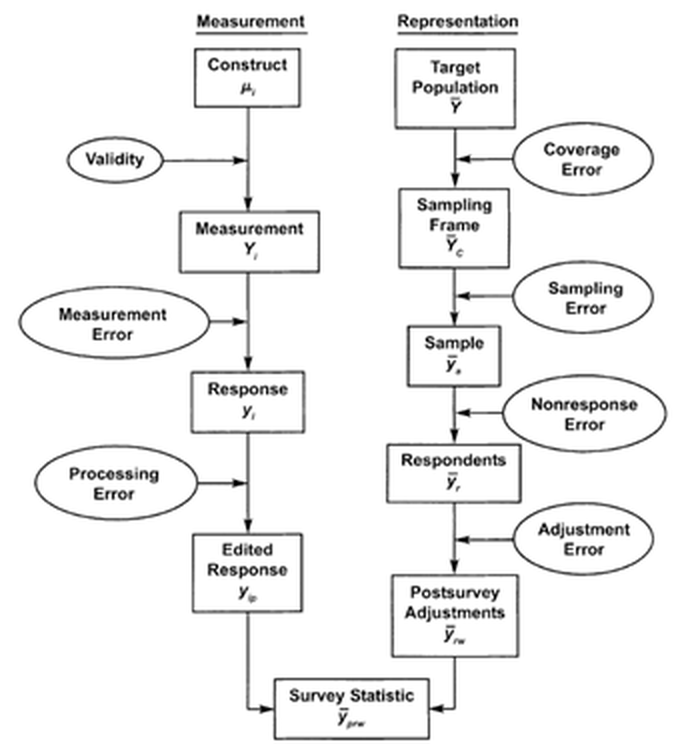
\includegraphics[width=\textwidth,height=0.72\textheight,keepaspectratio]{tse_groves.png}%
}{%
\resizebox{\textwidth}{!}{%
\begin{tikzpicture}[
  caja/.style={draw=pizarra, text=pizarra, thick, fill=pizarra!15, rounded corners=4pt, minimum width=2.3cm, minimum height=0.95cm, font=\sffamily\small, align=center, text width=2.1cm},
  errc/.style={draw=doradooscuro, text=doradooscuro, thick, fill=doradooscuro!15, rounded corners=4pt, font=\sffamily\scriptsize\bfseries, inner sep=3pt, align=center, text width=1.45cm, minimum height=0.95cm},
  paso/.style={-Stealth, thick, pizarra}]
  \node[font=\sffamily\bfseries, text=marino, anchor=west] at (-1.2,1.1) {MEDICIÓN: ¿qué medimos y qué tan bien?};
  \node[caja] (c1) at (0,0) {Constructo};
  \node[errc] (e1) at (2.1,0) {Validez};
  \node[caja] (c2) at (4.2,0) {Medición (pregunta)};
  \node[errc] (e2) at (6.3,0) {Error de medición};
  \node[caja] (c3) at (8.4,0) {Respuesta};
  \node[errc] (e3) at (10.5,0) {Error de proce\-samiento};
  \node[caja] (c4) at (12.6,0) {Respuesta editada};
  \foreach \a/\b in {c1/e1,e1/c2,c2/e2,e2/c3,c3/e3,e3/c4} \draw[paso] (\a) -- (\b);
  \node[font=\sffamily\bfseries, text=salvia, anchor=west] at (-1.2,-2.0) {REPRESENTACIÓN: ¿a quiénes medimos?};
  \node[caja] (r1) at (0,-3.1) {Población objetivo};
  \node[errc] (f1) at (2.1,-3.1) {Error de cobertura};
  \node[caja] (r2) at (4.2,-3.1) {Marco muestral};
  \node[errc] (f2) at (6.3,-3.1) {Error muestral};
  \node[caja] (r3) at (8.4,-3.1) {Muestra};
  \node[errc] (f3) at (10.5,-3.1) {Error de no respuesta};
  \node[caja] (r4) at (12.6,-3.1) {Respon\-dentes};
  \node[errc] (f4) at (14.7,-3.1) {Error de ajuste};
  \node[caja] (r5) at (16.8,-3.1) {Ajustes (ponderación)};
  \foreach \a/\b in {r1/f1,f1/r2,r2/f2,f2/r3,r3/f3,f3/r4,r4/f4,f4/r5} \draw[paso] (\a) -- (\b);
  \node[draw=marino, text=marino, fill=marino!15, thick, rounded corners=4pt, font=\sffamily\small\bfseries, align=center, text width=2.4cm, minimum height=0.95cm] (est) at (16.8,-1.55) {Estadístico de la encuesta};
  \draw[paso] (c4) -| (est);
  \draw[paso] (r5) -- (est);
\end{tikzpicture}}%
}
\fuente{Groves et al. (2009, cap.~2).}
\end{frame}

% ---------------------------------------------------------------------
\begin{frame}{Leyendo el mapa}
\begin{columns}[T]
\column{0.48\textwidth}
\begin{block}{Columna de medición}
\small
¿\textbf{Qué} medimos y \textbf{qué tan bien}? Va desde la idea teórica hasta el número en la base de datos
\end{block}
\column{0.48\textwidth}
\begin{exampleblock}{Columna de representación}
\small
¿\textbf{A quiénes} medimos? Va desde la población que nos interesa hasta quienes efectivamente respondieron
\end{exampleblock}
\end{columns}
\bigskip
\begin{itemize}
  \item Cada recuadro de error es un lugar donde podemos perder la verdad
  \item Los errores \textbf{se acumulan}: el estadístico final los hereda todos
  \item El margen de error que publica la prensa mide \textbf{solo} el error muestral
  \item Hoy nos concentramos en la \hl{columna de medición}
\end{itemize}
\end{frame}

% ---------------------------------------------------------------------
\begin{frame}{Errores de representación: ejemplos}
\begin{center}
\small
\begin{tabular}{>{\raggedright}p{0.17\textwidth}>{\raggedright}p{0.34\textwidth}p{0.39\textwidth}}
\toprule
\textbf{Error} & \textbf{¿Qué es?} & \textbf{Ejemplo} \\
\midrule
\rowcolor{crema}
Cobertura & El marco no incluye a toda la población & Encuesta por teléfono fijo: deja fuera a hogares sin línea fija \\
Muestral & Estudiar una muestra y no a todos & El ``margen de error $\pm 3$ puntos'' \\
\rowcolor{crema}
No respuesta & Quienes no responden son distintos & Personas con jornadas largas nunca están en casa \\
Ajuste & Ponderar mal para corregir lo anterior & Ponderar por sexo y edad cuando el sesgo es educacional \\
\bottomrule
\end{tabular}
\end{center}
\bigskip
\footnotesize Caso clásico: en 1936 la revista \textit{Literary Digest} encuestó a 2,4 millones de personas y predijo la derrota de Roosevelt, que ganó por amplio margen. Muchos casos no corrigen un mal marco ni una mala tasa de respuesta
\end{frame}

% ---------------------------------------------------------------------
\begin{frame}{Errores de medición: ejemplos}
\begin{center}
\small
\begin{tabular}{>{\raggedright}p{0.17\textwidth}>{\raggedright}p{0.36\textwidth}p{0.37\textwidth}}
\toprule
\textbf{Error} & \textbf{¿Qué es?} & \textbf{Ejemplo} \\
\midrule
\rowcolor{crema}
Validez & La pregunta no captura el concepto & Medir ``participación política'' solo con el voto \\
Medición & La respuesta se aleja del valor verdadero & ``¿Ha consumido drogas?'' preguntado frente a la familia \\
\rowcolor{crema}
Procesamiento & Errores al digitar, codificar o limpiar & Codificar ``trabaja en el retail'': ¿cajero? ¿gerente? \\
\bottomrule
\end{tabular}
\end{center}
\bigskip
\begin{alertblock}{Un error de procesamiento silencioso}
\small
Imaginen una escala codificada \code{1 Nada, 2 Poca, 3 Algo, 4 Bastante, 6 Mucha}. Si nadie lo detecta, todos los promedios de confianza quedan inflados
\end{alertblock}
\end{frame}

% ---------------------------------------------------------------------
\begin{frame}{Un mismo tema, tres encuestas, tres números}
\small
¿Qué piensan los chilenos sobre el MEPCO? (marzo--abril de 2026)
\bigskip

\begin{center}
\begin{tabular}{>{\raggedright}p{0.22\textwidth}>{\raggedright}p{0.5\textwidth}r}
\toprule
\textbf{Encuesta} & \textbf{Lo que se preguntó (en síntesis)} & \textbf{Resultado} \\
\midrule
\rowcolor{crema}
Cadem, Plaza Pública & El Gobierno debía endeudarse para mantener el subsidio & 48\% de acuerdo \\
Pulso Ciudadano & Rechazo a la decisión de \textbf{no} aplicar el mecanismo & 57,2\% rechaza \\
\rowcolor{crema}
Métrica Pública & Rechazo a la eliminación o suspensión del MEPCO & 65,5\% rechaza \\
\bottomrule
\end{tabular}
\end{center}
\bigskip
\begin{alertblock}{Para discutir}
\small
¿Estas encuestas se contradicen? ¿O cada una mide \hlr{una cosa distinta}: el endeudamiento, una decisión del Gobierno, la existencia del mecanismo?
\end{alertblock}
\fuente{Cifras según reportes de prensa; verificar en los informes originales de cada encuesta.}
\end{frame}

% ---------------------------------------------------------------------
\sintesis{
  \item\textcolor{dorado}{Nos vamos a equivocar: la pregunta científica es por cuánto y en qué dirección}
  \bigskip
  \item\textcolor{dorado}{El error aleatorio se compensa con más casos; el sistemático no}
  \bigskip
  \item\textcolor{dorado}{Toda respuesta es verdad más error: X = V + E}
  \bigskip
  \item\textcolor{dorado}{El error total viene de cómo preguntamos (medición) y de a quiénes (representación)}
}

% =====================================================================
\seccion{Parte 3}{Del concepto al número}

% ---------------------------------------------------------------------
\begin{frame}{¿Cómo se mide\ldots?}
\centering
\begin{tikzpicture}[scale=0.9]
  \foreach \t/\x/\y in {el amor/-4.5/1.1, la inteligencia/0/1.4, la confianza\\en los demás/4.5/1.1, el autoritarismo/-3/-0.6, la depresión/3/-0.6, la eficacia\\política/0/-1.6} {
    \node[lat, minimum width=2.9cm, minimum height=1.1cm, font=\sffamily\normalsize\bfseries] at (\x,\y) {\t};
  }
\end{tikzpicture}
\bigskip
\begin{itemize}
  \item Son conceptos \hl{latentes}: existen (o eso creemos), pero \textbf{no se observan directamente}
  \item No hay una regla para medir el autoritarismo como la hay para medir la estatura
  \item Solo observamos sus \textbf{manifestaciones}: lo que la gente dice, hace o responde
\end{itemize}
\end{frame}

% ---------------------------------------------------------------------
\begin{frame}{Operacionalización}
\begin{block}{Asún (2006, p.~69)}
\small
(a) Definir cuidadosamente un concepto no observable; (b) derivar consecuencias observables, los \hl{indicadores}; (c) medir los indicadores; (d) deducir de ellos el grado en que el objeto posee el concepto
\end{block}
\bigskip
\begin{columns}[c]
\column{0.55\textwidth}
\textbf{Ejemplo de otras ciencias}
\begin{itemize}
  \item La \textbf{edad de un árbol} (latente) se mide contando los \textbf{anillos del tronco} (indicador)
  \item Funciona porque la relación es \textbf{directa y estable}
  \item En ciencias sociales esa relación casi nunca es tan limpia
\end{itemize}
\column{0.4\textwidth}
\centering
\begin{tikzpicture}
  \foreach \r in {0.25,0.5,...,1.5} \draw[doradooscuro] (0,0) circle (\r);
  \fill[doradooscuro!40] (0,0) circle (0.12);
  \node[font=\footnotesize, text=pizarra] at (0,-1.9) {6 anillos $\Rightarrow$ 6 años};
\end{tikzpicture}
\end{columns}
\end{frame}

% ---------------------------------------------------------------------
\begin{frame}{Dos roles en la ciencia: teoría y medición}
\begin{columns}[T]
\column{0.48\textwidth}
\centering
\imagen{sheldon_leonard.jpg}{0.9\textwidth}{2.9cm}{Sheldon y Leonard, \textit{The Big Bang Theory}}
\smallskip

\raggedright\small
\begin{itemize}
  \item \textbf{Sheldon}, físico \textbf{teórico}: trabaja con conceptos y ecuaciones
  \item \textbf{Leonard}, físico \textbf{experimental}: diseña instrumentos para medir
\end{itemize}
\column{0.48\textwidth}
\centering
\imagen{higgs.jpg}{0.42\textwidth}{2.9cm}{Peter Higgs (físico teórico)}\hspace{0.04\textwidth}
\imagen{cern_atlas.jpg}{0.42\textwidth}{2.9cm}{Detector ATLAS del CERN (física experimental)}
\smallskip

\raggedright\small
\begin{itemize}
  \item 1964: Higgs propone una partícula \textbf{en teoría}
  \item 2012: el CERN logra \textbf{medirla}, 48 años después
\end{itemize}
\end{columns}
\medskip
\begin{block}{En sociología}
\small
Hay una \hl{fase teórica} (qué es el concepto) y una \textbf{fase empírica} (cómo se traduce en números). La operacionalización es el puente
\end{block}
\end{frame}

% ---------------------------------------------------------------------
\begin{frame}{Del concepto al número}
\centering
\begin{tikzpicture}[scale=0.9]
  \node[lat, minimum width=2.4cm, minimum height=1.2cm] (c) at (0,0) {Concepto};
  \foreach \i/\y in {1/1.4,2/0,3/-1.4} {
    \node[lat, minimum width=2.2cm, font=\sffamily\small] (d\i) at (3.6,\y) {Dimensión \i};
    \draw[flecha] (c) -- (d\i);
    \node[obs, minimum width=1.7cm, minimum height=0.45cm, font=\sffamily\scriptsize] (d\i a) at (7,\y+0.3) {Pregunta};
    \node[obs, minimum width=1.7cm, minimum height=0.45cm, font=\sffamily\scriptsize] (d\i b) at (7,\y-0.3) {Pregunta};
    \draw[flecha] (d\i) -- (d\i a.west); \draw[flecha] (d\i) -- (d\i b.west);
  }
  \node[lat, minimum width=1.6cm, minimum height=1.2cm] (i) at (10.4,0) {Índice\\\large 45};
  \foreach \i in {1,2,3} {\draw[flecha] (d\i a.east) -- (i.west); \draw[flecha] (d\i b.east) -- (i.west);}
  \draw[decorate, decoration={brace, amplitude=6pt, mirror}, thick, dorado] (-1.2,-2.3) -- (4.8,-2.3) node[midway, below=8pt, font=\sffamily\small\bfseries, text=doradooscuro] {Fase teórica};
  \draw[decorate, decoration={brace, amplitude=6pt, mirror}, thick, dorado] (5.6,-2.3) -- (11.3,-2.3) node[midway, below=8pt, font=\sffamily\small\bfseries, text=doradooscuro] {Fase empírica};
\end{tikzpicture}
\bigskip

\small Concepto $\rightarrow$ dimensiones $\rightarrow$ preguntas $\rightarrow$ categorías de respuesta $\rightarrow$ índice o escala
\fuente{Adaptado de Asún (2006, p.~75).}
\end{frame}

% ---------------------------------------------------------------------
\begin{frame}{Conceptos simples y conceptos complejos}
\begin{columns}[T]
\column{0.48\textwidth}
\begin{block}{Concepto simple}
\small
Las personas lo usan en su vida cotidiana \textbf{igual que el investigador}\\[4pt]
\footnotesize ``¿Cuántos años tiene?''\\
``¿Se siente enamorado de su pareja actual?''
\end{block}
\column{0.48\textwidth}
\begin{block}{Concepto complejo}
\small
El habla cotidiana \textbf{no lo usa}, o lo usa distinto\\[4pt]
\footnotesize No podemos preguntar ``¿cuán individuado está usted?''
\end{block}
\end{columns}
\bigskip
\begin{itemize}
  \item Operacionalizar un concepto complejo es un proceso de \hl{traducción}: del lenguaje del investigador al habla de las personas
  \item Hay que \textbf{desagregarlo} en dimensiones hasta llegar a algo que la gente pueda responder
\end{itemize}
\fuente{Asún (2006, pp.~71--73).}
\end{frame}

% ---------------------------------------------------------------------
\begin{frame}{Un ejemplo chileno: individuación (PNUD, 2002)}
\begin{center}
\small
\begin{tabular}{>{\raggedright}p{0.27\textwidth}p{0.64\textwidth}}
\toprule
\textbf{Dimensión} & \textbf{Pregunta} \\
\midrule
\rowcolor{crema}
Disposición a romper normas sociales & ¿Seguiría adelante con una idea aunque vaya en contra de la opinión de sus padres? ¿De su pareja? ¿De la Iglesia? \\
Deberes morales que restringen la conducta & ¿Cómo le gustaría ser recordado? (a) alguien que se entregó a los demás; (b) alguien que salió adelante contra viento y marea; (c) \textbf{alguien fiel a sus sueños}; (d) alguien que cumplió su deber \\
\rowcolor{crema}
Biografía como decisión personal & ¿Cuál frase lo representa mejor? (a) \textbf{Yo analizo mi vida y veo qué hacer}; (b) En la vida uno tiene que hacer lo que hay que hacer \\
\bottomrule
\end{tabular}
\end{center}
\medskip
Un punto por cada respuesta ``individualizada'' $\Rightarrow$ \hl{índice de 0 a 5}
\fuente{Ejemplo desarrollado en Asún (2006, pp.~73--75).}
\end{frame}

% ---------------------------------------------------------------------
\begin{frame}{Operacionalizar siempre tiene un costo}
\vfill
\begin{center}
\begin{minipage}{0.82\textwidth}
\large\itshape
``El proceso de operacionalización siempre implica un grado de distorsión o mutilación del sentido teórico de un concepto. [\ldots] Nunca logramos medir totalmente el concepto que buscamos, sólo obtenemos mejores o peores interpretaciones empíricas.''
\end{minipage}
\end{center}
\begin{flushright}\small Asún (2006, p.~77)\end{flushright}
\bigskip
\begin{block}{Pregunta al curso}
\small
¿Las cinco preguntas del PNUD capturan todo lo que un sociólogo entiende por ``individuación''? ¿Qué quedó fuera?
\end{block}
\vfill
\end{frame}

% ---------------------------------------------------------------------
\begin{frame}{Por qué usamos varias preguntas}
\begin{columns}[c]
\column{0.55\textwidth}
\begin{itemize}
  \item Cada pregunta trae su propio error: el fraseo, las palabras, el orden de las alternativas
  \item Si una pregunta empuja hacia arriba y otra hacia abajo, \hl{el promedio se acerca a la verdad}
  \item Es la lógica de ``más casos'', aplicada a \textbf{más ítems}
\end{itemize}
\bigskip
\begin{exampleblock}{Asún (2006, p.~91)}
\small
Si en una prueba de 60 preguntas un alumno capaz se confunde con una, su puntaje total igual reflejará su conocimiento
\end{exampleblock}
\column{0.4\textwidth}
\centering
\begin{tikzpicture}[scale=0.9]
  \node[lat] (V) at (0,2.6) {Concepto};
  \foreach \i/\x in {1/-1.8,2/-0.6,3/0.6,4/1.8} {
    \node[obs, minimum width=1cm, font=\sffamily\scriptsize] (x\i) at (\x,0.9) {ítem \i};
    \node[errn, minimum width=0.8cm, minimum height=0.6cm, font=\sffamily\scriptsize\bfseries] (e\i) at (\x,-0.5) {$e_\i$};
    \draw[flecha] (V) -- (x\i);
    \draw[flechae] (e\i) -- (x\i);
  }
  \node[font=\scriptsize, align=center, text=gris] at (0,-1.5) {los errores se compensan\\en el promedio};
\end{tikzpicture}
\end{columns}
\end{frame}

% ---------------------------------------------------------------------
\begin{frame}{Validez y confiabilidad}
\begin{columns}[T]
\column{0.48\textwidth}
\begin{block}{Confiabilidad}
\small
¿El instrumento entrega \textbf{el mismo resultado} si lo aplicamos dos veces a alguien que no ha cambiado?\\[4pt]
\footnotesize Una regla que hoy dice 15 cm y en cinco minutos dice 20 cm no sirve
\end{block}
\column{0.48\textwidth}
\begin{block}{Validez}
\small
¿El instrumento mide \textbf{lo que dice medir}?\\[4pt]
\footnotesize Si digo que mido autoritarismo, que sea autoritarismo y no otra cosa
\end{block}
\end{columns}
\bigskip
\centering
\begin{tikzpicture}[scale=0.55]
  \diana{0}{0}{}
  \foreach \x/\y in {1.0/0.9,1.1/0.8,0.9/1.05,1.05/1.0} \filldraw[fill=dorado, draw=white, thick] (\x,\y) circle (0.16);
  \node[font=\small, align=left, right, text=pizarra] at (2.2,0) {\hl{confiable pero no válido}:\\siempre medimos lo mismo\ldots\\pero no lo que queríamos};
\end{tikzpicture}
\fuente{Asún (2006, pp.~101--102).}
\end{frame}

% ---------------------------------------------------------------------
\begin{frame}{Dos maneras de relacionar concepto e indicadores}
\begin{columns}[T]
\column{0.48\textwidth}
\centering\textbf{Reflectivo}\\[0.2cm]
\begin{tikzpicture}[scale=0.9]
  \node[lat] (A) at (0,1.8) {Autoritarismo};
  \foreach \i/\x in {1/-1.6,2/0,3/1.6} {\node[obs, minimum width=1.2cm, font=\sffamily\scriptsize] (a\i) at (\x,0) {ítem \i}; \draw[flecha] (A) -- (a\i);}
\end{tikzpicture}\\[0.2cm]
\raggedright\footnotesize
El concepto \textbf{causa} las respuestas: si alguien es autoritario, tenderá a estar de acuerdo con todos los ítems. Los ítems \textbf{deben correlacionar}
\column{0.48\textwidth}
\centering\textbf{Formativo}\\[0.2cm]
\begin{tikzpicture}[scale=0.9]
  \node[lat] (C) at (0,1.8) {Calidad vivienda};
  \foreach \t/\x [count=\i] in {material/-1.7,servicios/0,entorno/1.7} {\node[obs, minimum width=1.4cm, font=\sffamily\scriptsize] (m\i) at (\x,0) {\t}; \draw[flecha] (m\i) -- (C);}
\end{tikzpicture}\\[0.2cm]
\raggedright\footnotesize
Los indicadores \textbf{componen} el concepto: una casa puede tener buen material y mal entorno. \textbf{No tienen por qué correlacionar}
\end{columns}
\bigskip
\begin{alertblock}{¿Por qué importa?}
\small
En un modelo formativo, eliminar el indicador ``que no correlaciona'' significa \hlr{amputar una parte del concepto}
\end{alertblock}
\fuente{Bollen \& Lennox (1991). El ejemplo de calidad de la vivienda está en Asún (2006, p.~76).}
\end{frame}

% ---------------------------------------------------------------------
\begin{frame}{¿Qué hace una persona cuando responde?}
\centering
\begin{tikzpicture}[scale=0.9]
  \foreach \t/\s/\x [count=\i] in {1. Comprensión/¿qué me preguntan?/0, 2. Recuperación/¿qué recuerdo?/3.6, 3. Juicio/¿qué pienso?/7.2, 4. Respuesta/¿qué alternativa elijo?/10.8} {
    \node[lat, minimum width=3cm, minimum height=1.3cm] (p\i) at (\x,0) {\t\\\footnotesize\mdseries \s};
  }
  \foreach \a/\b in {1/2,2/3,3/4} \draw[flecha] (p\a) -- (p\b);
  \foreach \i/\t in {1/{palabras difíciles\\dobles negaciones}, 2/{periodos vagos\\``últimamente''}, 3/{cansancio\\``cualquier cosa''}, 4/{deseabilidad social\\aquiescencia}} {
    \node[font=\scriptsize, text=doradooscuro, align=center, below=0.35cm of p\i] {\t};
  }
\end{tikzpicture}
\bigskip
\begin{itemize}
  \item En \textbf{cada etapa} algo puede salir mal (en dorado)
  \item Las reglas de redacción no son manías: cada una protege una etapa
  \item Si la tarea es difícil y la motivación baja, la gente responde ``lo suficiente'' (\textit{satisficing}, Krosnick, 1991)
\end{itemize}
\fuente{Tourangeau, Rips \& Rasinski (2000).}
\end{frame}

% ---------------------------------------------------------------------
\begin{frame}{Ejercicio: ¿qué tienen de malo estas preguntas?}
\begin{enumerate}
  \item ¿Está de acuerdo con que el gobierno aumente el sueldo mínimo y reduzca la jornada laboral?
  \item ¿No está usted en contra de que no se prohíba fumar en los parques?
  \item ¿Con qué frecuencia lee el diario? \quad {\footnotesize (Nunca / A veces / Frecuentemente)}
  \item ¿Cuánto se ha visto perjudicado por la delincuencia desatada que vive el país?
  \item ¿Cuál es su ingreso? \quad {\footnotesize (Menos de \$500 mil / \$500 mil a \$1 millón / \$1 a \$2 millones)}
  \item ¿Cuántas veces fue al médico el año pasado?
\end{enumerate}
\bigskip
\begin{block}{En parejas, 2 minutos}
\small
Identifiquen el problema de cada una y propongan una mejor versión
\end{block}
\end{frame}

% ---------------------------------------------------------------------
\begin{frame}{Respuestas: las reglas detrás del ejercicio}
\begin{center}
\small
\renewcommand{\arraystretch}{1.4}
\begin{tabular}{c>{\raggedright}p{0.3\textwidth}p{0.55\textwidth}}
\toprule
& \textbf{Problema} & \textbf{Regla} \\
\midrule
\rowcolor{crema}
1 & Pregunta doble & Una pregunta, una idea: ¿y si apoyo el sueldo pero no la jornada? \\
2 & Doble negación & Formular en positivo \\
\rowcolor{crema}
3 & Términos vagos & ``A veces'' significa cosas distintas para cada persona \\
4 & Sesgada y con presupuesto & ``Desatada'' carga la respuesta y asume un perjuicio \\
\rowcolor{crema}
5 & Categorías no exhaustivas ni excluyentes & ¿Y si gano \$3 millones? ¿Dónde queda \$1 millón exacto? \\
6 & Periodo ambiguo & ¿Año calendario o últimos 12 meses? \\
\bottomrule
\end{tabular}
\end{center}
\fuente{Lenzner \& Menold (2016), \emph{GESIS Survey Guidelines: Question Wording}; Asún (2006, pp.~80--90).}
\end{frame}

% ---------------------------------------------------------------------
\begin{frame}{Preguntar también produce la opinión}
\begin{columns}[T]
\column{0.55\textwidth}
\begin{itemize}
  \item Asún lo llama \hl{cristalización}: preguntar hace que la persona se sitúe donde antes no se había situado
  \item ``Cuando aplicamos un cuestionario estamos \emph{produciendo} información y no sólo \emph{recogiendo} información'' (p.~72)
\end{itemize}
\bigskip
\begin{exampleblock}{Una ley que no existía}
\small
En EE.UU. se preguntó si había que derogar la \textit{Public Affairs Act of 1975}, una ley \textbf{inventada}. Cerca de \textbf{un tercio} dio su opinión igual
\end{exampleblock}
\column{0.4\textwidth}
\begin{block}{Implicancias}
\small
\begin{itemize}
  \item Ofrecer la opción ``no sabe''
  \item Preguntar primero si conoce el tema
  \item Desconfiar de opiniones sobre temas poco conocidos
\end{itemize}
\end{block}
\end{columns}
\fuente{Bishop, Oldendick, Tuchfarber \& Bennett (1980), \emph{Public Opinion Quarterly}, 44(2).}
\end{frame}

% ---------------------------------------------------------------------
\sintesis{
  \item\textcolor{dorado}{Los conceptos sociológicos son latentes: solo vemos sus manifestaciones}
  \bigskip
  \item\textcolor{dorado}{Operacionalizar es traducir: concepto, dimensiones, preguntas, categorías, índice}
  \bigskip
  \item\textcolor{dorado}{Varias preguntas por concepto reducen el error aleatorio}
  \bigskip
  \item\textcolor{dorado}{Cada etapa de la respuesta puede fallar: las reglas de redacción la protegen}
}

% =====================================================================
\seccion{Parte 4}{Tres casos reales: ELSOC}

% ---------------------------------------------------------------------
\begin{frame}{ELSOC: Estudio Longitudinal Social de Chile}
\begin{columns}[c]
\column{0.55\textwidth}
\begin{itemize}
  \item Encuesta \hl{panel} del Centro de Estudios de Conflicto y Cohesión Social (COES)
  \item Sigue a \textbf{las mismas personas} año a año desde 2016
  \item Población urbana adulta de Chile
  \item Módulos: ciudadanía, desigualdad, redes, salud y bienestar, territorio, conflicto
  \item Cuestionarios, bases y documentación son \textbf{públicos}
  \item Sitio del estudio: \href{https://coes.cl/elsoc/}{\textcolor{azulmedio}{ELSOC -- COES}}
\end{itemize}
\column{0.4\textwidth}
\centering
\imagen{elsoc_terreno.jpg}{0.95\textwidth}{4.2cm}{Encuestador/a de ELSOC con tablet, o logo COES--ELSOC}
\end{columns}
\end{frame}

% ---------------------------------------------------------------------
\begin{frame}{La operacionalización, en una planilla}
\small
El \textit{Listado de Variables} de ELSOC documenta, para cada ítem, su concepto y su pregunta:
\bigskip

\begin{center}
\footnotesize
\begin{tabular}{l>{\raggedright}p{0.16\textwidth}>{\raggedright}p{0.16\textwidth}>{\raggedright}p{0.34\textwidth}l}
\toprule
\textbf{Código} & \textbf{Concepto general} & \textbf{Concepto específico} & \textbf{Fraseo del ítem} & \textbf{Tipo} \\
\midrule
\rowcolor{crema}
\code{c10\_02} & Autoeficacia política & Autoeficacia política & Mi voto influye en el resultado de la elección & Ordinal \\
\code{c18\_06} & Autoritarismo & Autoritarismo 1 & La obediencia y el respeto por la autoridad son los valores más importantes que los niños debieran aprender & Ordinal \\
\rowcolor{crema}
\code{s11\_02} & Estado de ánimo & Sintomatología depresiva & Decaimiento, pesadez o desesperanza & Ordinal \\
\bottomrule
\end{tabular}
\end{center}
\smallskip
Concepto $\rightarrow$ dimensión $\rightarrow$ pregunta $\rightarrow$ categorías: el diagrama de Asún, \hl{hecho planilla}
\fuente{ELSOC, Listado de Variables Global v2023.}
\end{frame}

% ---------------------------------------------------------------------
\begin{frame}{Caso 1. Autoeficacia política: la teoría}
\begin{columns}[c]
\column{0.55\textwidth}
\begin{itemize}
  \item \textbf{Eficacia política}: la sensación de que uno \textbf{puede} influir en la política (Campbell et al., 1954)
  \item Dos dimensiones clásicas:
  \begin{itemize}
    \item \hl{Interna}: ``entiendo la política y puedo participar''
    \item \textbf{Externa}: ``el sistema responde a gente como yo''
  \end{itemize}
  \item Un concepto vecino: el \textbf{deber cívico}, la sensación de que \emph{hay que} participar
\end{itemize}
\column{0.4\textwidth}
\centering
\begin{tikzpicture}[scale=0.9]
  \node[lat, minimum width=2.8cm] (E) at (0,2) {Eficacia política};
  \node[lat, minimum width=1.6cm, font=\sffamily\scriptsize\bfseries] (I) at (-1.4,0.3) {Interna};
  \node[lat, minimum width=1.6cm, font=\sffamily\scriptsize\bfseries] (X) at (1.4,0.3) {Externa};
  \draw[flecha] (E) -- (I); \draw[flecha] (E) -- (X);
  \node[obs, font=\sffamily\scriptsize\bfseries] (D) at (0,-1.3) {Deber cívico};
  \node[font=\scriptsize, text=gris] at (0,-2) {(concepto vecino)};
\end{tikzpicture}
\end{columns}
\fuente{Campbell, Gurin \& Miller (1954); Niemi, Craig \& Mattei (1991).}
\end{frame}

% ---------------------------------------------------------------------
\begin{frame}{Caso 1. Autoeficacia política en ELSOC}
\begin{center}
``¿En qué medida se encuentra usted de acuerdo o en desacuerdo con cada una de las siguientes afirmaciones?''
\end{center}
\medskip
\begin{center}
\begin{tabular}{lp{0.55\textwidth}}
\toprule
\rowcolor{crema}
\code{c10\_01} & Votar es mi deber como ciudadano \\
\code{c10\_02} & Mi voto influye en el resultado de la elección \\
\rowcolor{crema}
\code{c10\_03} & Votar permite expresar mis ideas \\
\bottomrule
\end{tabular}
\end{center}
\centering\footnotesize Totalmente en desacuerdo -- En desacuerdo -- Ni de acuerdo ni en desacuerdo -- De acuerdo -- Totalmente de acuerdo
\bigskip
\begin{block}{Pregunta al curso}
\small
\raggedright ¿Qué \textbf{faceta} de la relación con el voto captura cada ítem?
\end{block}
\end{frame}

% ---------------------------------------------------------------------
\begin{frame}{Caso 1. Una escala corta, varias facetas}
\centering
\begin{tikzpicture}[scale=0.9]
  \node[lat, minimum width=5cm] (A) at (0,2.4) {Relación con el voto};
  \node[lat, font=\sffamily\small\bfseries, minimum width=2.8cm] (DC) at (-4.4,0.9) {Deber cívico};
  \node[lat, font=\sffamily\small\bfseries, minimum width=2.8cm] (EF) at (0,0.9) {Eficacia del voto};
  \node[lat, font=\sffamily\small\bfseries, minimum width=2.8cm] (EX) at (4.4,0.9) {Valor expresivo};
  \draw[flecha] (A) -- (DC); \draw[flecha] (A) -- (EF); \draw[flecha] (A) -- (EX);
  \node[obs, text width=3.2cm] (i1) at (-4.4,-0.6) {\code{c10\_01}\\Votar es mi deber};
  \node[obs, text width=3.2cm] (i2) at (0,-0.6) {\code{c10\_02}\\Mi voto influye};
  \node[obs, text width=3.2cm] (i3) at (4.4,-0.6) {\code{c10\_03}\\Votar expresa ideas};
  \draw[flecha] (DC) -- (i1); \draw[flecha] (EF) -- (i2); \draw[flecha] (EX) -- (i3);
\end{tikzpicture}
\bigskip
\begin{itemize}
  \item Una encuesta panel cubre \textbf{muchos} temas: cada concepto recibe pocas preguntas
  \item Asún: el mínimo es una o dos preguntas por subconcepto; el resto se ``invierte'' en los conceptos centrales del estudio (p.~92)
  \item Cada ítem aporta \hl{una faceta}: quien analiza los datos decide cuáles usar según su pregunta
\end{itemize}
\end{frame}

% ---------------------------------------------------------------------
\begin{frame}{Caso 1. Leer la documentación antes de analizar}
\begin{columns}[T]
\column{0.5\textwidth}
\begin{exampleblock}{Lo que permite una buena documentación}
\small
\begin{itemize}
  \item Ver el fraseo exacto de cada ítem
  \item Elegir los ítems que calzan con \textbf{mi} concepto
  \item Saber en qué olas se preguntó cada uno
\end{itemize}
\end{exampleblock}
\bigskip
\begin{block}{Ejemplo}
\small
Si me interesa la eficacia \textbf{externa}, \code{c10\_02} es mi mejor candidato; si me interesa la cultura cívica, \code{c10\_01}
\end{block}
\column{0.46\textwidth}
\begin{alertblock}{La lección}
\small
La \hlr{etiqueta} de una variable es un punto de partida, no una garantía. La validez se juzga \textbf{en relación con la pregunta de investigación} de quien usa los datos
\end{alertblock}
\bigskip
\small
Que ELSOC publique concepto, fraseo y olas de cada ítem es justamente lo que hace posible esta discusión
\end{columns}
\end{frame}

% ---------------------------------------------------------------------
\begin{frame}{Caso 1. ¿Por qué importa medirlo bien?}
\begin{columns}[c]
\column{0.5\textwidth}
\begin{itemize}
  \item Verba, Schlozman \& Brady (1995): no todos tienen la misma \hl{voz política}
  \item Participar requiere \textbf{recursos} (tiempo, dinero, habilidades), \textbf{compromiso} (interés, eficacia) y \textbf{redes} que te recluten
  \item La eficacia es parte del mecanismo por el cual la \textbf{desigualdad social se vuelve desigualdad política}
\end{itemize}
\column{0.47\textwidth}
\centering
\begin{tikzpicture}[scale=0.9]
  \node[obs] (NSE) at (0,2.2) {Nivel socioeconómico\\y educación};
  \node[lat] (EF) at (-1.6,0.4) {Eficacia};
  \node[obs] (R) at (1.7,0.4) {Recursos\\(tiempo, dinero)};
  \node[obs] (P) at (0,-1.4) {\textbf{Participación}};
  \draw[flecha] (NSE) -- (EF); \draw[flecha] (NSE) -- (R);
  \draw[flecha] (EF) -- (P); \draw[flecha] (R) -- (P);
\end{tikzpicture}
\end{columns}
\bigskip
\begin{alertblock}{Medir no es solo un problema técnico}
\small
Cómo medimos la eficacia define qué podemos decir sobre \textbf{un mecanismo de la desigualdad}
\end{alertblock}
\end{frame}

% ---------------------------------------------------------------------
\begin{frame}{Caso 2. Autoritarismo: una larga historia}
\begin{columns}[c]
\column{0.58\textwidth}
\begin{itemize}
  \item Adorno, Frenkel-Brunswik, Levinson \& Sanford (1950), \textit{The Authoritarian Personality}
  \item Pregunta tras el nazismo: ¿por qué personas comunes apoyan regímenes autoritarios?
  \item Construyeron la \hl{escala F} (de ``fascismo''): obediencia, convencionalismo, agresión hacia los desviados
  \item Incluía preguntas sobre la relación con los padres, justificadas desde la \textbf{teoría psicoanalítica} (Asún, 2006, p.~112)
\end{itemize}
\column{0.38\textwidth}
\centering
\imagen{adorno_authoritarian.jpg}{0.9\textwidth}{4.6cm}{Portada de \textit{The Authoritarian Personality} (1950) o foto de T. W. Adorno}
\end{columns}
\end{frame}

% ---------------------------------------------------------------------
\begin{frame}{Caso 2. Autoritarismo en ELSOC}
\small
``¿En qué medida se encuentra usted de acuerdo o en desacuerdo con cada una de las siguientes afirmaciones?''
\medskip

\begin{center}
\begin{tabular}{lp{0.72\textwidth}}
\toprule
\rowcolor{crema}
\code{c18\_04} & En vez de tanta preocupación por los derechos de las personas, lo que este país necesita es un gobierno firme \\
\code{c18\_05} & Lo que nuestro país necesita es un mandatario/a fuerte con la determinación para llevarnos por el camino correcto \\
\rowcolor{crema}
\code{c18\_06} & La obediencia y el respeto por la autoridad son los valores más importantes que los niños debieran aprender \\
\code{c18\_07} & Las verdaderas claves para tener una buena vida son la obediencia y la disciplina \\
\bottomrule
\end{tabular}
\end{center}
\medskip
\begin{block}{Miren con atención}
\small
¿Qué significa responder ``de acuerdo'' en \textbf{las cuatro} afirmaciones?
\end{block}
\end{frame}

% ---------------------------------------------------------------------
\begin{frame}{Caso 2. Un desafío de toda escala de acuerdo/desacuerdo}
\begin{itemize}
  \item En los cuatro ítems, \textbf{estar de acuerdo = más autoritario}
  \item Es el formato estándar de muchas escalas, desde la escala F hasta encuestas internacionales actuales
  \item Su riesgo: la \hl{aquiescencia}, la tendencia a responder ``de acuerdo'' \textbf{independientemente del contenido}
\end{itemize}
\bigskip
\begin{columns}[T]
\column{0.48\textwidth}
\begin{block}{¿Por qué ocurre?}
\small
\begin{itemize}
  \item Cortesía con el encuestador
  \item Deferencia hacia quien pregunta
  \item Menor esfuerzo: es más fácil buscar razones para estar de acuerdo (Krosnick, 1991)
\end{itemize}
\end{block}
\column{0.48\textwidth}
\begin{alertblock}{Consecuencia}
\small
Una persona aquiescente puede aparecer como \textbf{más autoritaria} de lo que es: un \hlr{error sistemático}
\end{alertblock}
\end{columns}
\fuente{Bogner \& Landrock (2016), \emph{GESIS Survey Guidelines: Response Biases in Standardised Surveys}, sección 2.2.}
\end{frame}

% ---------------------------------------------------------------------
\begin{frame}{Caso 2. El DAG del problema}
\centering
\begin{tikzpicture}[scale=0.9]
  \node[lat, minimum width=2.8cm] (A) at (0,0) {Autoritarismo};
  \node[obs, minimum width=2.8cm] (R) at (6.4,0) {Puntaje en\\la escala};
  \node[errn, minimum width=2.8cm] (Q) at (6.4,2.4) {Aquiescencia};
  \node[obs, minimum width=2.8cm] (Ed) at (0,2.4) {Educación};
  \draw[flecha] (A) -- (R);
  \draw[flechae] (Q) -- (R);
  \draw[flechad] (Ed) -- node[midway, below=4pt, font=\scriptsize, text=doradooscuro, align=center] {menos educación,\\más aquiescencia} (Q);
  \draw[flecha] (Ed) -- node[left, font=\small, text=pizarra] {?} (A);
\end{tikzpicture}
\bigskip
\begin{itemize}
  \item Si las personas con menos educación aparecen ``más autoritarias'', ¿cuánto es autoritarismo y cuánto es \textbf{forma de responder}?
  \item El error de medición puede \hl{fabricar o inflar relaciones} entre variables
\end{itemize}
\end{frame}

% ---------------------------------------------------------------------
\begin{frame}{Caso 2. ¿Cómo se enfrenta?}
\begin{columns}[T]
\column{0.32\textwidth}
\begin{block}{1. Escalas balanceadas}
\small
Mitad de los ítems en un sentido y mitad en el otro: la aquiescencia se cancela\\[3pt]
\footnotesize Ej.: escala RWA de Altemeyer
\end{block}
\column{0.32\textwidth}
\begin{block}{2. Categorías propias}
\small
Reemplazar ``de acuerdo / en desacuerdo'' por alternativas del ítem\\[3pt]
\footnotesize ``¿Cuánto influye su voto?'' Nada -- Poco -- Algo -- Mucho
\end{block}
\column{0.32\textwidth}
\begin{block}{3. Medición indirecta}
\small
Preguntar por otra cosa que revela el concepto\\[3pt]
\footnotesize ¿Qué es más importante que aprenda un niño: \textbf{obediencia} o \textbf{independencia}? (Feldman \& Stenner, 1997)
\end{block}
\end{columns}
\bigskip
\begin{itemize}
  \item La opción 3 elige entre dos cosas \textbf{deseables}: no hay un ``de acuerdo'' fácil
  \item Medir bien exige \hl{creatividad conceptual}, no solo técnica
\end{itemize}
\fuente{Bogner \& Landrock (2016); Saris, Revilla, Krosnick \& Shaeffer (2010); Feldman \& Stenner (1997).}
\end{frame}

% ---------------------------------------------------------------------
\begin{frame}{Caso 3. Depresión: un instrumento clínico en una encuesta}
\small
``¿Cuántas veces durante las \textbf{últimas dos semanas} ha sentido alguna de las siguientes molestias?''
\medskip

\begin{columns}[T]
\column{0.6\textwidth}
\footnotesize
\renewcommand{\arraystretch}{1.2}
\begin{tabular}{lp{0.7\textwidth}}
\toprule
\rowcolor{crema} \code{s11\_01} & Poco interés o alegría para realizar sus actividades \\
\code{s11\_02} & Decaimiento, pesadez o desesperanza \\
\rowcolor{crema} \code{s11\_03} & Dificultad para dormir, o exceso de sueño \\
\code{s11\_04} & Cansancio o falta de energía \\
\rowcolor{crema} \code{s11\_05} & Apetito disminuido o aumentado \\
\code{s11\_06} & Dificultad para concentrarse \\
\rowcolor{crema} \code{s11\_07} & Mala opinión de sí mismo \\
\code{s11\_08} & Movimientos o lenguaje enlentecidos \\
\rowcolor{crema} \code{s11\_09} & Pensamientos de muerte o de hacerse daño \\
\bottomrule
\end{tabular}
\column{0.36\textwidth}
\begin{block}{PHQ-9}
\small
\begin{itemize}
  \item \textit{Patient Health Questionnaire}: instrumento clínico validado
  \item Nueve síntomas, periodo de referencia preciso
  \item Asún: \hl{no inventar todo}, usar instrumentos probados (p.~108)
\end{itemize}
\end{block}
\end{columns}
\end{frame}

% ---------------------------------------------------------------------
\begin{frame}{Caso 3. Adaptar tiene costos}
\begin{columns}[c]
\column{0.48\textwidth}
\textbf{PHQ-9 original} (4 categorías)
\begin{itemize}
  \item[0] Nunca
  \item[1] Varios días
  \item[2] Más de la mitad de los días
  \item[3] Casi todos los días
\end{itemize}
\column{0.48\textwidth}
\textbf{ELSOC} (5 categorías)
\begin{itemize}
  \item[1] Nunca
  \item[2] Algunos días
  \item[3] Más de la mitad de los días
  \item[4] Casi todos los días
  \item[5] \hld{Todos los días}
\end{itemize}
\end{columns}
\bigskip
\begin{itemize}
  \item El PHQ-9 tiene \textbf{puntajes de corte} (5, 10, 15, 20) para la escala 0--27
  \item Con otra escala de respuesta, esos cortes no se aplican directamente
  \item Toda adaptación es una decisión con costos y beneficios de \hl{comparabilidad}
\end{itemize}
\end{frame}

% ---------------------------------------------------------------------
\begin{frame}{Caso 3. El problema de tener a alguien enfrente}
\begin{columns}[c]
\column{0.5\textwidth}
\begin{itemize}
  \item Responder sobre el propio ánimo frente a un \textbf{desconocido} no es neutral
  \item \hl{Deseabilidad social}: responder lo que ``queda bien''
  \item \textbf{Efecto encuestador}: las respuestas cambian según quién pregunta
  \item \textbf{Presencia de terceros}: la pareja o los hijos en la sala
\end{itemize}
\column{0.47\textwidth}
\centering
\begin{tikzpicture}[scale=0.9]
  \node[lat] (D) at (0,0) {Síntomas\\reales};
  \node[obs] (R) at (3.6,0) {Síntomas\\declarados};
  \node[errn, font=\sffamily\scriptsize\bfseries] (Enc) at (3.6,2.2) {Encuestador\\presente};
  \node[errn, font=\sffamily\scriptsize\bfseries] (Ter) at (0.4,2.2) {Terceros\\presentes};
  \draw[flecha] (D) -- (R);
  \draw[flechae] (Enc) -- (R);
  \draw[flechae] (Ter) -- (R);
\end{tikzpicture}
\\[0.2cm]
\footnotesize Ambos empujan \textbf{hacia abajo}: subreporte
\end{columns}
\fuente{Bogner \& Landrock (2016), secciones 2.1, 3.1 y 3.2.}
\end{frame}

% ---------------------------------------------------------------------
\begin{frame}{Caso 3. La solución de ELSOC: pasar la tablet}
\begin{columns}[c]
\column{0.55\textwidth}
\begin{itemize}
  \item En este módulo el encuestador \textbf{entrega la tablet} y la persona responde sola
  \item ELSOC lo registra: \code{s11\_10} indica si la persona contestó directamente en la tablet
  \item Lo mismo con el \textbf{voto}: ``PREGUNTA AUTOADMINISTRADA. ENTREVISTADO DEBE RESPONDER DIRECTAMENTE EN LA TABLET''
\end{itemize}
\bigskip
\begin{exampleblock}{Asún ya lo anticipaba (p.~108)}
\small
Aumentar la confidencialidad ``dejando que parte del instrumento lo responda secretamente (sin mediación del encuestador)''
\end{exampleblock}
\column{0.4\textwidth}
\centering
\imagen{tablet_autoaplicada.jpg}{0.95\textwidth}{4.4cm}{Persona respondiendo sola en una tablet (encuesta autoaplicada)}
\end{columns}
\end{frame}

% ---------------------------------------------------------------------
\begin{frame}{Caso 3. Una pregunta abierta: ¿qué es la depresión?}
\begin{columns}[T]
\column{0.48\textwidth}
\centering\textbf{Causa común}\\[0.2cm]
\begin{tikzpicture}[scale=0.9]
  \node[lat] (D) at (0,1.6) {Depresión};
  \foreach \t/\x [count=\i] in {ánimo/-2.4,sueño/-0.8,energía/0.8,concentr./2.4} {\node[obs, minimum width=1.3cm, font=\sffamily\scriptsize] (s\i) at (\x,0) {\t}; \draw[flecha] (D) -- (s\i);}
\end{tikzpicture}\\[0.2cm]
\raggedright\footnotesize
La depresión es una condición latente que \textbf{produce} los síntomas: sumarlos tiene sentido
\column{0.48\textwidth}
\centering\textbf{Red de síntomas}\\[0.2cm]
\begin{tikzpicture}[scale=0.9]
  \node[obs, minimum width=1.3cm, font=\sffamily\scriptsize] (s) at (-1.6,1.6) {sueño};
  \node[obs, minimum width=1.3cm, font=\sffamily\scriptsize] (e) at (1.6,1.6) {energía};
  \node[obs, minimum width=1.3cm, font=\sffamily\scriptsize] (c) at (1.6,0) {concentr.};
  \node[obs, minimum width=1.3cm, font=\sffamily\scriptsize] (a) at (-1.6,0) {ánimo};
  \draw[flecha] (s) -- (e); \draw[flecha] (e) -- (c); \draw[flecha] (c) -- (a); \draw[flecha] (a) -- (s);
\end{tikzpicture}\\[0.2cm]
\raggedright\footnotesize
Los síntomas \textbf{se causan entre sí}: la depresión \emph{es} la red. Ojo: este dibujo \textbf{no es un DAG}, porque tiene un ciclo
\end{columns}
\bigskip
\begin{block}{La lección}
\small
Incluso en instrumentos clínicos, \hl{¿qué es el concepto?} sigue siendo una pregunta abierta. Operacionalizar es tomar posición teórica
\end{block}
\fuente{Borsboom \& Cramer (2013); Fried \& Nesse (2015).}
\end{frame}

% ---------------------------------------------------------------------
\begin{frame}{Caso 3. Medir también tiene consecuencias éticas}
\begin{itemize}
  \item El ítem \code{s11\_09} pregunta por \textbf{pensamientos de muerte o de hacerse daño}
  \item Una encuesta que pregunta esto debe estar preparada para lo que puede escuchar:
  \begin{itemize}
    \item protocolos de \hl{derivación} a apoyo profesional
    \item encuestadores capacitados
    \item aprobación de un \textbf{comité de ética}
  \end{itemize}
\end{itemize}
\bigskip
\begin{center}
\small
\begin{tabular}{lll}
\toprule
\textbf{Caso} & \textbf{Pregunta} & \textbf{Fuente de error} \\
\midrule
\rowcolor{crema}
Autoeficacia & ¿qué faceta mide cada ítem? & validez \\
Autoritarismo & ¿el formato empuja? & sesgo de respuesta \\
\rowcolor{crema}
Depresión & ¿la situación empuja? & efecto encuestador y modo \\
\bottomrule
\end{tabular}
\end{center}
\end{frame}

% ---------------------------------------------------------------------
\sintesis{
  \item\textcolor{dorado}{Una buena documentación permite discutir la validez de cada ítem}
  \bigskip
  \item\textcolor{dorado}{El formato de acuerdo/desacuerdo puede introducir error sistemático}
  \bigskip
  \item\textcolor{dorado}{La situación de entrevista cambia las respuestas: la autoaplicación protege los temas sensibles}
  \bigskip
  \item\textcolor{dorado}{Toda medición es también una posición teórica y una responsabilidad ética}
}

% =====================================================================
\seccion{Parte 5}{Innovaciones: experimentos, modos y datos vinculados}

% ---------------------------------------------------------------------
\begin{frame}{Experimentos dentro de encuestas}
\begin{columns}[c]
\column{0.52\textwidth}
\begin{itemize}
  \item Se asigna \hl{al azar} a cada persona una versión distinta del cuestionario
  \item Como el azar decide, los grupos son \textbf{comparables en todo lo demás}
  \item Cualquier diferencia en las respuestas se debe a \textbf{la versión}
  \item Combina \textbf{muestras representativas} con \textbf{inferencia causal}
\end{itemize}
\column{0.45\textwidth}
\centering
\begin{tikzpicture}[scale=0.9]
  \node[lat] (Z) at (0,2.2) {Azar};
  \node[obs] (V) at (0,0.4) {Versión\\A / B};
  \node[obs] (Y) at (3.4,0.4) {Respuesta};
  \node[obs, font=\sffamily\scriptsize] (U) at (3.4,2.2) {Edad, educación,\\ideología\ldots};
  \draw[flecha] (Z) -- (V); \draw[flecha] (V) -- (Y); \draw[flecha] (U) -- (Y);
  \draw[flechad] (U) -- (V) node[pos=0.5, font=\Large\bfseries, text=doradooscuro] {$\times$};
\end{tikzpicture}
\\[0.2cm]
\footnotesize El azar \textbf{corta} la flecha entre las características de las personas y la versión que reciben
\end{columns}
\fuente{Mutz (2011), \emph{Population-Based Survey Experiments}.}
\end{frame}

% ---------------------------------------------------------------------
\begin{frame}{Dos experimentos clásicos de fraseo}
\begin{columns}[T]
\column{0.48\textwidth}
\begin{exampleblock}{Prohibir vs. permitir (Rugg, 1941)}
\small
``¿Debería EE.UU. \textbf{prohibir} los discursos públicos contra la democracia?'' $\rightarrow$ 54\% sí\\[4pt]
``¿Debería \textbf{permitir}\ldots?'' $\rightarrow$ 75\% no\\[4pt]
Misma idea, \textbf{21 puntos} de diferencia
\end{exampleblock}
\column{0.48\textwidth}
\begin{exampleblock}{Rangos de respuesta (Schwarz et al., 1985)}
\small
Horas diarias de televisión:\\[4pt]
Rangos \textbf{bajos} $\rightarrow$ 16\% dice más de 2½ horas\\
Rangos \textbf{altos} $\rightarrow$ 38\% dice más de 2½ horas\\[4pt]
Las alternativas sugieren qué es ``normal''
\end{exampleblock}
\end{columns}
\bigskip
\begin{itemize}
  \item Ambos son \textit{split-ballot}: dos versiones asignadas al azar
  \item El primero muestra error en una \textbf{opinión}; el segundo, en un \hl{hecho}
\end{itemize}
\end{frame}

% ---------------------------------------------------------------------
\begin{frame}{Tipos de experimentos en encuestas}
\begin{center}
\small
\begin{tabular}{>{\raggedright}p{0.17\textwidth}>{\raggedright}p{0.43\textwidth}p{0.32\textwidth}}
\toprule
\textbf{Diseño} & \textbf{En qué consiste} & \textbf{Sirve para} \\
\midrule
\rowcolor{crema}
\textit{Split-ballot} & Dos redacciones de la misma pregunta & Efectos de fraseo, orden, escalas \\
Viñetas & Historias breves con atributos que varían (sexo, clase, nacionalidad\ldots) & Juicios de justicia, discriminación, merecimiento \\
\rowcolor{crema}
\textit{Conjoint} & Elegir entre perfiles que combinan varios atributos & Preferencias por candidatos, políticas, inmigrantes \\
Lista & Contar cuántas afirmaciones de una lista son ciertas; un grupo tiene una extra sensible & Temas sensibles: compra de votos, discriminación \\
\bottomrule
\end{tabular}
\end{center}
\fuente{Auspurg \& Hinz (2015); Hainmueller, Hopkins \& Yamamoto (2014); Blair \& Imai (2012).}
\end{frame}

% ---------------------------------------------------------------------
\begin{frame}{Así se ve un \textit{conjoint}}
\begin{columns}[c]
\column{0.58\textwidth}
\centering
\fcolorbox{pizarra}{white}{\begin{minipage}{0.92\textwidth}
\vspace{4pt}
\footnotesize
\textbf{Pantalla 3 de 5.} Considere a estos dos candidatos a alcalde:
\medskip

\centering
\renewcommand{\arraystretch}{1.3}
\begin{tabular}{lcc}
\toprule
& \textbf{Candidato A} & \textbf{Candidato B} \\
\midrule
\rowcolor{crema}
Edad & 38 años & 61 años \\
Género & Mujer & Hombre \\
\rowcolor{crema}
Profesión & Profesora & Empresario \\
Experiencia & Concejal 8 años & Ninguna \\
\rowcolor{crema}
Prioridad & Seguridad & Vivienda \\
\bottomrule
\end{tabular}
\medskip

\raggedright
Si tuviera que elegir, ¿por cuál votaría?\quad $\bigcirc$ A \quad $\bigcirc$ B
\vspace{4pt}
\end{minipage}}
\column{0.38\textwidth}
\begin{itemize}
  \item Los atributos se asignan \hl{al azar} en cada pantalla
  \item La persona repite la elección varias veces
  \item Se estima cuánto pesa cada atributo en la decisión
  \item Útil cuando la gente no reconoce sus preferencias, por ejemplo de género
\end{itemize}
\end{columns}
\fuente{Ejemplo ficticio. Hainmueller, Hopkins \& Yamamoto (2014).}
\end{frame}

% ---------------------------------------------------------------------
\begin{frame}{Modos de aplicación y \textit{mixed-mode}}
\begin{columns}[c]
\column{0.55\textwidth}
\begin{itemize}
  \item El \textbf{mismo cuestionario no mide igual} cara a cara, por teléfono o por web
  \item Teléfono: preguntas cortas, pocas alternativas, sin tarjetas
  \item Web o autoaplicado: más reporte de temas sensibles, pero nadie aclara dudas
  \item \hl{Mixed-mode}: combinar modos para reducir costos o no respuesta, a riesgo de mezclar \textbf{efectos de modo}
\end{itemize}
\column{0.4\textwidth}
\begin{exampleblock}{Caso chileno: CASEN 2020}
\small
Por la pandemia, se aplicó mayoritariamente por \textbf{teléfono}, con un cuestionario reducido. El Ministerio advirtió cautela al comparar con años anteriores
\end{exampleblock}
\bigskip
\footnotesize La tablet de ELSOC es un \textbf{cambio de modo dentro de la misma entrevista}
\end{columns}
\fuente{de Leeuw (2005); Kreuter, Presser \& Tourangeau (2008).}
\end{frame}

% ---------------------------------------------------------------------
\begin{frame}{Más allá del cuestionario: vincular datos}
\centering
\begin{tikzpicture}[scale=0.85]
  \node[lat, minimum width=3cm, minimum height=1.3cm] (E) at (0,0) {Respuestas\\de la encuesta};
  \node[obs, text width=4.4cm, minimum height=1.3cm] (A) at (-5.6,1.5) {\textbf{Registros administrativos}\\\scriptsize trayectoria educativa (MINEDUC), Registro Social de Hogares (MDSF)};
  \node[obs, text width=4.4cm, minimum height=1.3cm] (Q) at (5.6,1.5) {\textbf{Seguimiento cualitativo}\\\scriptsize ¿acepta ser contactado para una entrevista en profundidad?};
  \node[obs, text width=4.4cm, minimum height=1.3cm] (D) at (-5.6,-1.5) {\textbf{Donación de datos}\\\scriptsize la persona descarga y entrega su historial de Instagram o LinkedIn};
  \node[obs, text width=4.4cm, minimum height=1.3cm] (P) at (5.6,-1.5) {\textbf{Paradatos}\\\scriptsize tiempos de respuesta, cambios de respuesta, dispositivo};
  \foreach \n in {A,Q,D,P} \draw[flecha, Stealth-Stealth] (\n) -- (E);
\end{tikzpicture}
\bigskip
\begin{itemize}
  \item La encuesta deja de ser la única fuente: se \hl{conecta} con otros datos sobre la misma persona
  \item Permite medir hechos sin depender del recuerdo y combinar métodos cuantitativos y cualitativos
\end{itemize}
\end{frame}

% ---------------------------------------------------------------------
\begin{frame}{Un ejemplo real: ELSOC pide el RUT}
\begin{columns}[T]
\column{0.58\textwidth}
\begin{exampleblock}{Pregunta \code{m66\_01} (cuestionario 2022)}
\small
``Con el objetivo de potenciar el desarrollo de estudios y políticas públicas basadas en evidencia [\ldots] queremos consultarle sobre la posibilidad de contar con su RUT, de manera de poder \textbf{vincular sus respuestas} en esta encuesta con datos administrativos [\ldots] ¿Compartiría usted su RUT para fines de este estudio?''
\end{exampleblock}
\bigskip
\small
La pregunta recuerda los protocolos de confidencialidad y la aprobación del \textbf{comité de ética}
\column{0.38\textwidth}
\begin{alertblock}{Condiciones éticas}
\small
\begin{itemize}
  \item Consentimiento \hlr{específico} para cada vínculo
  \item Derecho a decir que no sin consecuencias
  \item Datos seudonimizados y resguardados
  \item Aprobación de un comité de ética
\end{itemize}
\end{alertblock}
\bigskip
\footnotesize Quienes aceptan vincular sus datos pueden ser distintos de quienes no: otra fuente de error de representación
\end{columns}
\fuente{ELSOC, cuestionario maestro 2022; Sakshaug \& Kreuter (2012); Boeschoten et al. (2022).}
\end{frame}

% ---------------------------------------------------------------------
\sintesis{
  \item\textcolor{dorado}{Los experimentos en encuestas combinan muestras representativas con inferencia causal}
  \bigskip
  \item\textcolor{dorado}{Split-ballot, viñetas, conjoint y listas permiten estudiar el fraseo y los temas sensibles}
  \bigskip
  \item\textcolor{dorado}{El modo de aplicación también es parte de la medición}
  \bigskip
  \item\textcolor{dorado}{Vincular encuestas con registros, entrevistas y datos digitales exige consentimiento y resguardo ético}
}

% ---------------------------------------------------------------------
\begin{frame}{Recomendaciones para construir un cuestionario}
\begin{columns}[T]
\column{0.5\textwidth}
\begin{enumerate}
  \item \textbf{No inventar todo}: revisar instrumentos existentes (ELSOC, CEP, CASEN, ISSP)
  \item \textbf{Varias preguntas} por concepto importante
  \item Seguir las \textbf{reglas de redacción}
  \item Pensar el \textbf{orden}: de lo simple a lo complejo, lo sensible al final
\end{enumerate}
\column{0.5\textwidth}
\begin{enumerate}\setcounter{enumi}{4}
  \item Temas sensibles: \textbf{autoaplicación} y confidencialidad
  \item \textbf{Pretest}: probar con personas reales y preguntar cómo entendieron
  \item Trabajar en \textbf{equipo}
  \item \hl{No esperar perfección}: ``en toda encuesta siempre hay preguntas que no funcionan'' (Asún, p.~67)
\end{enumerate}
\end{columns}
\fuente{Asún (2006, pp.~66--67, 98--100, 108--109).}
\end{frame}

% ---------------------------------------------------------------------
\begin{frame}{Un recurso para seguir: GESIS Survey Guidelines}
\begin{columns}[c]
\column{0.55\textwidth}
\centering
\imagen{gesis_guidelines.png}{\textwidth}{5.2cm}{Pantallazo del índice de las GESIS Survey Guidelines}
\column{0.42\textwidth}
\begin{itemize}
  \item Guías breves del instituto alemán GESIS, con \textbf{revisión de pares}
  \item De \hl{acceso libre} (licencia CC BY-NC)
  \item Una guía para cada decisión:
  \begin{itemize}
    \item redacción de preguntas
    \item diseño de escalas
    \item sesgos de respuesta
    \item pretest cognitivo
    \item modos de aplicación
  \end{itemize}
\end{itemize}
\end{columns}
\end{frame}

% ---------------------------------------------------------------------
\sintesis{
  \item\textcolor{dorado}{Trabajar con datos es obsesionarse con el error: nos vamos a equivocar, la pregunta es por cuánto}
  \bigskip
  \item\textcolor{dorado}{El error viene de a quiénes preguntamos y de cómo preguntamos}
  \bigskip
  \item\textcolor{dorado}{Los conceptos sociológicos son latentes: medirlos exige traducirlos con cuidado}
  \bigskip
  \item\textcolor{dorado}{Operacionalizar es una decisión teórica, no solo técnica}
  \bigskip
  \item\textcolor{dorado}{Fraseo, formato y situación de entrevista cambian las respuestas, y podemos estudiarlo}
}

% ---------------------------------------------------------------------
\begin{frame}[allowframebreaks]{Referencias}
\tiny
\begin{itemize}
\item[] Adorno, T. W., Frenkel-Brunswik, E., Levinson, D. \& Sanford, N. (1950). \emph{The Authoritarian Personality}. Harper.
\item[] Asún, R. (2006). Construcción de cuestionarios y escalas: El proceso de la producción de información cuantitativa. En M. Canales (Ed.), \emph{Metodologías de investigación social} (pp.~63--114). LOM.
\item[] Auspurg, K. \& Hinz, T. (2015). \emph{Factorial Survey Experiments}. Sage.
\item[] Bishop, G., Oldendick, R., Tuchfarber, A. \& Bennett, S. (1980). Pseudo-opinions on public affairs. \emph{Public Opinion Quarterly}, 44(2), 198--209.
\item[] Blair, G. \& Imai, K. (2012). Statistical analysis of list experiments. \emph{Political Analysis}, 20(1), 47--77.
\item[] Boeschoten, L., Ausloos, J., Möller, J., Araujo, T. \& Oberski, D. (2022). A framework for privacy preserving digital trace data collection through data donation. \emph{Computational Communication Research}, 4(2), 388--423.
\item[] Bogner, K. \& Landrock, U. (2016). \emph{Response Biases in Standardised Surveys}. GESIS Survey Guidelines.
\item[] Bollen, K. \& Lennox, R. (1991). Conventional wisdom on measurement: A structural equation perspective. \emph{Psychological Bulletin}, 110(2), 305--314.
\item[] Borsboom, D. \& Cramer, A. (2013). Network analysis: An integrative approach to the structure of psychopathology. \emph{Annual Review of Clinical Psychology}, 9, 91--121.
\item[] Campbell, A., Gurin, G. \& Miller, W. (1954). \emph{The Voter Decides}. Row, Peterson.
\item[] de Leeuw, E. (2005). To mix or not to mix data collection modes in surveys. \emph{Journal of Official Statistics}, 21(2), 233--255.
\item[] Feldman, S. \& Stenner, K. (1997). Perceived threat and authoritarianism. \emph{Political Psychology}, 18(4), 741--770.
\item[] Fried, E. \& Nesse, R. (2015). Depression sum-scores don't add up. \emph{BMC Medicine}, 13, 72.
\item[] Groves, R., Fowler, F., Couper, M., Lepkowski, J., Singer, E. \& Tourangeau, R. (2009). \emph{Survey Methodology} (2ª ed.). Wiley.
\item[] Hainmueller, J., Hopkins, D. \& Yamamoto, T. (2014). Causal inference in conjoint analysis. \emph{Political Analysis}, 22(1), 1--30.
\item[] Jackman, S. \& Spahn, B. (2019). Why does the ANES overestimate voter turnout? \emph{Political Analysis}, 27(2), 193--207.
\item[] Kreuter, F., Presser, S. \& Tourangeau, R. (2008). Social desirability bias in CATI, IVR, and Web surveys. \emph{Public Opinion Quarterly}, 72(5), 847--865.
\item[] Krosnick, J. (1991). Response strategies for coping with the cognitive demands of attitude measures in surveys. \emph{Applied Cognitive Psychology}, 5(3), 213--236.
\item[] Lenzner, T. \& Menold, N. (2016). \emph{Question Wording}. GESIS Survey Guidelines.
\item[] Mutz, D. (2011). \emph{Population-Based Survey Experiments}. Princeton University Press.
\item[] Niemi, R., Craig, S. \& Mattei, F. (1991). Measuring internal political efficacy in the 1988 National Election Study. \emph{American Political Science Review}, 85(4), 1407--1413.
\item[] Pearl, J. \& Mackenzie, D. (2018). \emph{The Book of Why}. Basic Books.
\item[] Rugg, D. (1941). Experiments in wording questions: II. \emph{Public Opinion Quarterly}, 5(1), 91--92.
\item[] Sakshaug, J. \& Kreuter, F. (2012). Assessing the magnitude of non-consent biases in linked survey and administrative data. \emph{Survey Research Methods}, 6(2), 113--122.
\item[] Saris, W., Revilla, M., Krosnick, J. \& Shaeffer, E. (2010). Comparing questions with agree/disagree response options to questions with item-specific response options. \emph{Survey Research Methods}, 4(1), 61--79.
\item[] Schwarz, N., Hippler, H.-J., Deutsch, B. \& Strack, F. (1985). Response scales: Effects of category range on reported behavior and comparative judgments. \emph{Public Opinion Quarterly}, 49(3), 388--395.
\item[] Stevens, S. S. (1946). On the theory of scales of measurement. \emph{Science}, 103(2684), 677--680.
\item[] Tourangeau, R., Rips, L. \& Rasinski, K. (2000). \emph{The Psychology of Survey Response}. Cambridge University Press.
\item[] Verba, S., Schlozman, K. \& Brady, H. (1995). \emph{Voice and Equality: Civic Voluntarism in American Politics}. Harvard University Press.
\end{itemize}
\end{frame}

% ---------------------------------------------------------------------
\begin{frame}[plain]
  \vspace{0.5cm}
  {\usebeamerfont{title}\color{marino}\inserttitle\par}
  \vspace{0.2cm}
  {\usebeamerfont{subtitle}\color{gris}\insertsubtitle\par}
  \vspace{0.3cm}
  {\color{dorado}\rule{0.6\textwidth}{1pt}\par}
  \vspace{0.6cm}
  {\insertauthor\par}\vspace{0.1cm}
  {\small aplazareveco@gmail.com\par}\vspace{0.1cm}
  {\small\href{https://alejandroplazareveco.github.io/}{\textcolor{doradooscuro}{alejandroplazareveco.github.io}}\par}
\end{frame}

\end{document}
